% The "%" character denotes a comment
% This file was written by Nathan Moore, Winona State University
% as a template for how lab reports might be written in LaTeX.
% style choices originally come from the American Journal of Physics's
% sample submission file, http://ajp.dickinson.edu/Contributors/manFormat.html
%
%
\documentclass[prb,preprint]{revtex4-1}
\usepackage{amsmath}  % needed for \tfrac, \bmatrix, etc.
\usepackage{amsfonts} % needed for bold Greek, Fraktur, and blackboard bold
\usepackage{graphicx} % needed for figures

%these are some macros (shortcuts)
\newcommand{\bea}{\begin{eqnarray}}
\newcommand{\eea}{\end{eqnarray}}
\newcommand{\be}{\begin{equation}}
\newcommand{\ee}{\end{equation}}

\begin{document}

\title{Operational Amplifier Circuits}
\author{Autumn Rasmussen}


\date{\today}

%if you include an abstract, it goes here
\begin{abstract}
In this laboratory, an operational amplifier was utilized to explore three basic operational amplifier circuits and the effects of changing a load resistance on the overall voltage gain of the amplifier.
\end{abstract}

\maketitle


%These are my general reccomendations for an undergraduate lab report in Physics. 
%
%\textbf{Purpose}
%The lab report should start with a purpose statement.  Briefly 
%provide the necessary background and explain what problem your are trying to 
%solve/investigate.
%
%\textbf{Conclusions} Don't be coy, cut to the point right away and state what you found. This should be breif.
%
%\textbf{Theory} We never just measure stuff in Physics.  There's always a 
%theoretical idea behind the measurement we're making.  Explain  the ideas 
%behind your work, starting at the level of a successful Physics 221/222 
%student.
%
%\textbf{Data} Sketch out, in words and pictures, the apparatus you used to take data.  Report the data, graphically, if possible, and state the uncertainties  in your measurement.  Don't provide pages of computer printout here. Data tables shouldn't be your first choice when it comes to communicating your measurements.\cite{Tufte}
%
%\textbf{Analysis} With data presented, describe how the theory agrees/disagrees with 
%the data you took.  Normally this is accomplished with a fit line (or math 
%model) that is interpreted.
%
%\textbf{Limitations and Recommendations} Every measurement has limitations and it is only honest to report them to the reader.  ``Human Error'' is a meaningless statement.  After your analysis is complete, revisit the purpose statement.  This is the place to more forcefully argue your conclusions.    
%
%Notes: 
%Writing in the first person, eg ``I" or ``We," is fine.
%\newpage
%\textbf{Example Lab Report:}
\section{Purpose}
An operational amplifier, also called an op amp, is a very commonly used device in electronics.
It embodies an electronic circuit, but can be treated as a black box devide where its terminal values are considered rather than the composition of its circuit. Op amps can control the voltage and current of a circuit such that by changing the types and arrangement of the feedback elements, different analog operations- addition, subtraction, multiplication, integration and differentiation- are implemented. This lab explores three basic operational amplifier circuits- inverting amplifier, voltage follower, and non-inverting amplifier- as well as the effects of changing the load resistance on the overall gain of the amplifier.

\section{Conclusions}
The measured results obtained are within error of the theoretical values for a given configuration.
This suggests that the op amps used can be considered ideal in the configurations we used. 

\section{Theory}
The LMF411 has eight terminals, five of them being utilized in this lab- positive power supply $(V^+)$, negative power supply $(V^-)$ , inverting input $(V_{-})$, non-inverting input $(V_{+})$, and output $(V_{out})$. Following the principles for an ideal op amp- the input impedance of $(V_{-})$ and $(V_{+})$ is infinite and theree is no voltage difference between  $(V_{-})$ and $(V_{+})$- theoretical gain can be derived for each circuit.\\

Within the inverting amplifier configuration, shown in \ref{fig1}, the input voltage is connected to the inverting input while the non-inverting input is connected to ground, resulting in a gain. From Ohm's Law and Kirchoff's Current Law, it is clear that
\be A_v=\frac{V_{out}}{V_{-}} = \frac{-Rf}{R1} \label{eq1} \ee such that the output voltage is inverted with respect to the input voltage. \\
 
\begin{figure} [ht]
\centering
\includegraphics[width=1.5in]{lab3_invertingopamp.png}
\caption{Inverting Op Amp Configuration}
\label{fig1}
\end{figure}

Within the voltage follower configuration, shown in \ref{fig2}, the input voltage is connected to the non-inverting input while the inverting input is connected to the output and to ground, resulting in a gain. It is clear that 
\be A_v=\frac{V_{out}}{V_{-}} = 1 \label{eq2} \ee such that there is a unity gain. \\

\begin{figure} [ht]
\centering
\includegraphics[width=1.5in]{lab3_voltagefollower.png}
\caption{ Op Amp Voltage Follower Configuration}
\label{fig2}
\end{figure}

%Within the non_inverting amplifier configuration, shown in \ref{fig3}, the input voltage is connected to the non-inverting input while the inverting input is connected to the output and to ground by resistors, resulting in a positive gain. From Ohm's Law and Kirchoff's Current Law, it is clear that
\be A_v=\frac{V_{out}}{V_{-}} = 1+ \frac{Rf}{R2} \label{eq3} \ee.  \\

\begin{figure} [ht]
\centering
\includegraphics[width=1.5in]{lab3_noninvertingopamp.png}
\caption{Non-Inverting Op Amp Configuration}
\label{fig3}
\end{figure}

\section{Data}
%The theory, equation \ref{eq1}, predicts voltage gain for the inverting amplifier. Using 1K\ohm resistors for Rf and R1, I verified that the voltage gain for this circuit is -1.0 by applying various DC voltages to the input, careful not to run into the op amp rails, and recorded the output. Output was also measured when Rf had a value of 10k\ohm and 20k\ohm. Results are shown \ref{Table 1}.

\begin{table}[h!]
\begin{center}
 \begin{tabular}{||c c c c||} 
 \hline
\textbf{V_{in} & V_{out} & A_v (theoretical) & A_v (actual) & percent error} \\ 
 \hline\hline
 2.04 & -2.04 & -1 & -1 & 0 \\ 
 \hline
 1.53 & -1.53 & -1 & -1 & 0\
 \hline
 1.15 & -1.15 & -1 & -1 & 0 \\
 \hline
 6.97 & -6.97 & -1 & -1 & 0\\
 \hline
 3.06 & -3.06 & -1 & -1 & 0\\ 
 \hline
 .26 & -2.62 & -10 & -10.07 & 0.7 \\ 
 \hline
 .26 & -5.24 & -20 & -20.15 & 0.75\\ 
 \hline
\end{tabular}
\end{center}
\caption{ Inverting Amplifier Results}
\label{Table 1}
\end{table}

The theory, equation \ref{eq2}, predicts voltage gain for the voltage follower configuration to be 1 by applying a DC voltage to the input, careful not to run into the op amp rails, and recorded the output. Results are shown \ref{Table 2}.

\begin{center}
 \begin{tabular}{||c c c c c||} 
 \hline
 V_{in} & V_{out} & V_{out}-V_{in} & A_v (actual) & percent error \\ [0.5ex] 
 \hline\hline
 .29 & .3 & 0.1 & 1.03 & 3 \\ 
 \hline
 4.37 & 4.37 & 0 & 1 & 0\\
 \hline
 7.59 & 7.62 & .03 & 1 & 0\\
 \hline
 10.9 & 10.9 & 0 & 1 & 0\\
 \hline
 9.54 & 9.55 & .01 & 1 &0\\ [1ex] 
 \hline
\end{tabular}
\end{center}
\caption{Voltage Follower Results}
\label{Table 2}\\

The theory, equation \ref{eq3}, predicts voltage gain for the non-inverting amplifier. To yield a voltage gain of +4, chose $Rf=3k\ohm$ and $R1= 1k\ohm$ by applying a DC voltage to the input, careful not to run into the op amp rails, and recorded the output.Results are shown \ref{Table 3}.

\begin{center}
 \begin{tabular}{||c c c c||} 
 \hline
 V_{in} & V_{out} & A_v (actual) & percent error \\ [0.5ex] 
 \hline\hline
 1.3 & 4.3 & 4 &0\\ [1ex] 
\end{tabular}
\end{center}
\caption{ Non-Inverting Amplifier Results}
\label{Table 3}\\
 
 
\section{Analysis}
Equation \ref{eq4} represents line in \ref{fig4}.  \be V_{out}=A_v(V_{in}) \label{eq4} \ee indicating that $V_{out} and V_{in} are directly proportional as shown in \ref{fig4} such that op-amp gain does not depend on the amplitude of the voltage signal, but rather the ratio of the amplitudes.


\begin{figure}[ht]
\centering
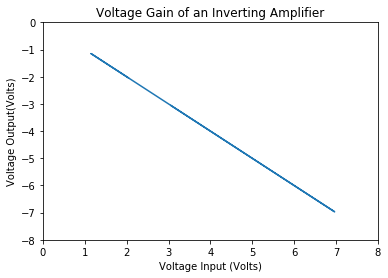
\includegraphics[width=\columnwidth]{lab3_python.png}
\caption{V_{out} vs. V_{in}}
\label{fig4}
\end{figure}
}

\end{document}
